
\begin{minipage}{.25\linewidth}
	\centering
	Hohlleiter
	\bigskip

	\def\r{1.8}
	\tdplotsetmaincoords{70}{120}
	\begin{tikzpicture}[tdplot_main_coords]
		% Drawing XYZ coordinates system
		\def \lenX {1.0*\r}
		\def \lenY {1.0*\r}
		\def \lenZ {0.3*\r}
		\def \boxX{.7*\r}
		\def \boxY{.9*\r}
		\def \boxZ{.2*\r}
		% Calculate box corner length
		\pgfmathsetmacro{\boxCornerLen}{sqrt{((\boxX)^2 + (\boxY)^2 + (\boxZ)^2)}}
		% Draw coordinate system
		\draw[dashed] (0,0,0) -- (\boxX,0,0);
		\draw[-stealth,thin] (\boxX,0,0) -- (\lenX,0,0) node[left] {$y$};
		\draw[dashed] (0,0,0) -- (0,\boxY,0);
		\draw[-stealth,thin] (0,\boxY,0) -- (0,\lenY,0) node[anchor=north west] {$z$};
		\draw[dashed] (0,0,0) -- (0,0,\boxZ);
		\draw[-stealth,thin] (0,0,\boxZ) -- (0,0,\lenZ) node[anchor=south] {$x$};

		% Drawing horizontal box:
		% Get corner polar coordinate
		\tdplotgetpolarcoords{\boxX}{\boxY}{\boxZ}
		\tdplotsetcoord{Box}{\boxCornerLen}{\tdplotrestheta}{\tdplotresphi}
		% Draw a box
		\draw[] (Boxx) -- (Boxxy);
		\draw[very thick] (Boxy) -- (Boxxy);
		\draw[] (Boxx) -- (Boxxz);
		\draw[] (Boxz) -- (Boxxz);
		\draw[very thick] (Boxy) -- (Boxyz);
		\draw[] (Boxz) -- (Boxyz);
		\draw[very thick] (Boxxy) -- (Box);
		\draw[] (Boxxz) -- (Box);
		\draw[very thick] (Boxyz) -- (Box);
	\end{tikzpicture}

\end{minipage}
\begin{minipage}{.25\textwidth}
	\centering
	Koaxialkabel

	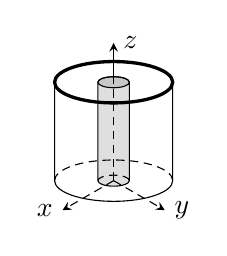
\begin{tikzpicture}
		\draw [fill=gray, fill opacity=.25] (180:2mm) coordinate (a)
		-- ++(0,-12.5mm) coordinate (b)
		arc (180:360:2mm and .7mm) coordinate (d) % 2 war 5
		-- (a -| d) coordinate (c) arc (0:180:2mm and .7mm); % 2 war 5
		\draw [fill=gray, fill opacity=.25]
		(0,0) coordinate (t) circle (2mm and .7mm);
		\draw [densely dashed] (d) arc (0:180:2mm and .7mm);
		\draw []
		(180:7.5mm) coordinate (A)
		-- ++(0,-12.5mm) coordinate (B)
		arc (180:360:7.5mm and 2.625mm) coordinate (D)
		-- (A -| D) coordinate (C) arc (0:180:7.5mm and 2.625mm);
		\draw [very thick]
		(0,0) coordinate (T) circle (7.5mm and 2.625mm);
		\draw [densely dashed] (D) arc (0:180:7.5mm and 2.625mm);
		\draw [densely dashed ]
		([yshift=-12.5mm]T) coordinate (B)
		edge [-stealth] node [pos=1, right] {$y$} +(-30:7.5mm)
		edge [-stealth] node [pos=1, left] {$x$} +(-150:7.5mm)
		-- (T) edge [solid, -stealth] node [right, pos=1] {$z$} ++(0,5mm) ;
	\end{tikzpicture}

\end{minipage}
\begin{minipage}{.25\textwidth}
	\centering
	Zweidrahtleitung (Lecher-Leitung)

	\begin{tikzpicture}
		\node [thick,cylinder, draw, shape border rotate=90,minimum height=1.5cm,minimum width=2mm] at (0,0){};
		\node [thick,cylinder, draw, shape border rotate=90,minimum height=1.5cm,minimum width=2mm] at (1cm,0cm){};
		\draw[thin, -stealth] (0.5cm,-0.80cm) -- (0.5cm,1cm) node[above]{$z$};
	\end{tikzpicture}
\end{minipage}
\begin{minipage}{.25\textwidth}
	\centering
	Mikrostreifenleitung
	\bigskip

	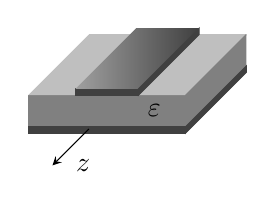
\begin{tikzpicture}[scale=0.4]
		\draw [lightgray] (0,1,0) coordinate (bl) -- (5,1,0) coordinate (br);
		\filldraw [gray] (0,0,5) coordinate (fll) -- (0,1,5) coordinate (ftl) -- (5,1,5) coordinate (ftr) -- (5,0,5) coordinate (flr) -- cycle;
		\shade [left color = lightgray, right color = lightgray] (bl) -- (br) -- (ftr) -- (ftl) -- cycle;
		\filldraw [gray] (5,0,0) coordinate (blr) -- (flr) -- (ftr) -- (br);
		\filldraw [darkgray] (fll) rectangle (5,-0.2,5) coordinate (flr2);
		\filldraw [darkgray] (flr2) -- (5,-0.2,0) coordinate (blr2) -- (blr) -- (flr) -- cycle;
		\filldraw [darkgray] (1.5,1.2,5) coordinate (ftl-1) -- (3.5,1.2,5) coordinate (ftr-1) -- (3.5,1,5) coordinate (flr-1) -- (1.5,1,5) coordinate (fll-1) -- cycle;
		\shade [left color = darkgray!50, right color = darkgray] (1.5,1.2,0) coordinate (btl-1) -- (3.5,1.2,0) coordinate (btr-1) -- (ftr-1) -- (ftl-1) -- cycle;
		\filldraw [darkgray] (flr-1) -- (ftr-1) -- (btr-1) --  (br -| btr-1) -- cycle;
		\node at (4,0.5,5) {$\varepsilon$};
		\coordinate (nA1) at (1.5,2.5,0);
		\coordinate (nB1) at (3.5,2.5,0);
		\coordinate (nA2) at (-1.5,1.2,0);
		\coordinate (nB2) at (-1.5,1.2,5);
		\coordinate (nA3) at (7,1,5);
		\coordinate (nB3) at (7,1.2,5);
		\coordinate (nA4) at (-1.5,1,5);
		\coordinate (nB4) at (-1.5,0,5);
		\draw[-stealth,thin] (0,-2,0) -- (0,-2,3) node[right,xshift=5]{$z$};
	\end{tikzpicture}

\end{minipage}